%-----------------------------------------------------------------------------%
%Packages%
\documentclass{beamer}
\usepackage{tikz}
\usepackage{comment}

\usetikzlibrary{arrows,shapes,automata}

% Drawings of frames

\tikzstyle{vertex}=[circle,fill=black!25,minimum size=20pt,inner sep=0pt]
\tikzstyle{selected vertex} = [vertex, fill=red!24]
\tikzstyle{edge} = [draw,thick,->]
\tikzstyle{weight} = [font=\small]

\pgfdeclarelayer{background}
\pgfsetlayers{background,main}

%-----------------------------------------------------------------------------%
%Document%
\begin{document}
\title{A Logical Framework for realising Action Model Execution}
\author{Edwin Tay}

\begin{comment}
My honours presentation.
Need to discuss project and give a motivating idea.
In general:

given an epistemic goal we can find an action model we can construct an
action model

given an epistemic action model how can we realise it

do no maths, use pictures

don’t say “this is too complicated” - don’t
mention the “too complicated stuff”!
\end{comment}

\frame{\titlepage}

\begin{frame}
\frametitle{Wanna play a game...?}
\begin{itemize}
  \item Consider two agents, Amy ($A$) and Brian ($B$)
  \item There's a coin in front of them, but they don't know whether the coin is
    Heads or Tails...
  \item We can model this as $\ldots$
\end{itemize}
\end{frame}

\begin{frame}
\begin{figure}
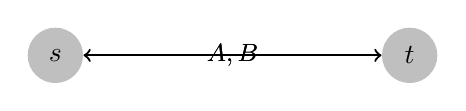
\begin{tikzpicture}[scale=1.5]

  \foreach \pos/\name in {{(0,0)/s}, {(3,0)/t}}
    \node[vertex] (\name) at \pos {$\name$};
  \foreach \source/\dest/\weight in {s/t/{A,B},t/s/{A,B}}
    \path[edge] (\source) -- node[weight] {$\weight$} (\dest);

\end{tikzpicture}
\end{figure}
\end{frame}

\end{document}
